\section{Projektplan}

\subsubsection*{Zweck dieses Dokuments}
Dieses Dokument beschreibt den Projektplan des Projekts «Methode 635 als Cross Plattform App mit Xamarin». Es beinhaltet die Planung, die Organisation sowie weitere Aspekte und liefert damit eine gute Übersicht über das Projekt. Es dient daher als Grundlage für den Verlauf des Projekts.

\subsubsection*{Gültigkeitsbereich}
Der Gültigkeitsbereich erstreckt sich über die gesamte Dauer des Projekts. Der Zeitraum geht vom 17. September 2018 bis zum 21. Dezember 2018. Das Projekt findet im Rahmen des Moduls «Studienarbeit» im Herbstsemester 2018 statt.

\subsection{Projektziel}
Die Motivation dieser Studienarbeit besteht darin, eine Cross-Platform App zu programmieren, welche die Methode 635 \cite{methode-635} als mobile App für Android und iOS umsetzt. Dabei sollen moderne Technologien zum Einsatz kommen, welche es den Anwendern ermöglichen schneller und einfacher eine Lösung für ein Problem zu erarbeiten.

\subsubsection*{Einschränkungen}
Das Projekt ist auf die Dauer des Herbstsemester 2018 begrenzt (bis 21. Dezember 2018). Zudem sollte das Projekt mit ungefähr 240 Arbeitsstunden (gesamthaft 480 Stunden) realisiert werden können. Bleibt am Ende Zeit übrig, werden optionale Features implementiert und als zusätzliche Funktionalität ergänzt.

\subsection{Projektorganisation}
In unserem Projekt arbeiten wir in einer flachen Organisationsstruktur, wobei die wesentlichen Entscheide im ganzen Projektteam und/oder mit dem Dozenten an den wöchentlichen Besprechungen getroffen werden. An den Besprechungen getroffene Entscheidungen werden in \href{https://github.com/BrainingOutOfBox/Doc/wiki} {Protokollen} dokumentiert. Die Projektmitglieder sind innerhalb des Teams gleichgestellt.

\subsubsection*{Organisationsstruktur}
Die Projektmitglieder sowie deren Verantwortung sind der Abbildung \ref{fig:organisation} zu entnehmen.
\begin{figure}[h]
	\centering
	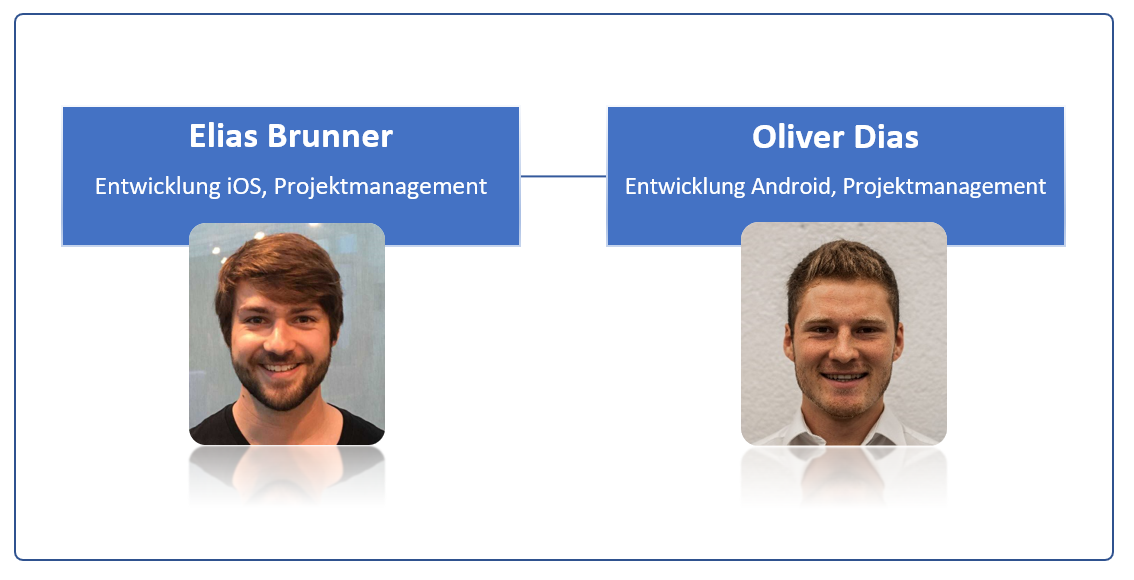
\includegraphics[width=1\linewidth]{img/projekt-plan/organisation}
	\caption[Organisation BrainingOutOfBox]{Braining Out Of Box Organisation}
	\label{fig:organisation}
\end{figure}

\subsubsection*{Ansprechspartner}
Im Projekt «Methode 635 als Cross Plattform App mit Xamarin» ist folgender Ansprechpartner vorhanden.

\begin{description}[leftmargin=!,labelwidth=\widthof{\bfseries Dozent}]
	\item[Dozent] Prof. Dr. Olaf Zimmermann ist der betreuende Dozent für diese Studienarbeit. Er ist neben der Betreuung auch für die Bewertung des Projekts verantwortlich. 
\end{description}

\subsection{Projektmanagement}
Eine ausführliche Iterationsplanung mit den dazugehörigen Meilensteinen befindet sich auf \href{https://hsr-sa.atlassian.net/}{Jira}. Die aufgewendeten Zeiten für ein Issue werden ebenfalls dort erfasst.


Da wir mit einer agilen Entwicklung arbeiten, wird die Planung während dem Projekt laufend aktualisiert und den aktuellen Gegebenheiten angepasst. 

Wie in Abbildung \ref{fig:projekt-plan} zu sehen, ist ein grober Projektablauf ausgearbeitet. 


%TODO: Repos sollten bald private sein
Zur Verwaltung des Codes nutzen wir \href{https://github.com/BrainingOutOfBox/App}{öffentliche Github Repositories}. Die Kommunikation abseits der HSR Anwesenheit erfolgt über einen Whats-App Chat oder alternativ über einen Slack Channel.

\subsubsection*{Besprechungen}
Das Projektteam trifft sich einmal in der Woche das ganze um sich über den aktuellen Stand des Projekts auszutauschen, Fragen zu klären, Probleme anzugehen oder die nächsten Schritte zu planen. 

Diese wöchentlichen Besprechungen finden, falls nicht anders vorgesehen, jeden Donnerstagmorgen um 09:00 Uhr statt. 

Über jede Besprechung wird \href{https://github.com/BrainingOutOfBox/Doc/wiki} {Protokoll} geführt. Dies mit dem Ziel, die Entscheidungen festzuhalten und Missverständnisse zu vermeiden.


\subsubsection*{Umgang mit Risiken}
Um auch auf unbekannte Risiken vorbereitet zu sein, ist am Ende des Projektes eine Reserve eingeplant. Zudem haben sich alle Teilnehmer bereit erklärt ihr Engagement punktuell zu erhöhen, falls die Situation dies erfordert. Diese Erhöhung sollte jedoch nur Phasenweise sein und in einer folgenden Phase kompensiert werden. 

Die häufigsten Risiken wurden mit einer Risikotabelle (Unterkapitel \ref{risiko-tabelle} ) be\-rück\-sichtigt, die aktuell gehalten wird und beim Planen in Betracht gezogen wird. 

\subsubsection*{Qualitätsmassnahmen}
Das Endprodukt dieses Projekts soll von möglichst hoher Qualität sein. Wie in Tabelle \ref{tab:Massnahmen} zu sehen ist, treffen wir folgende Massnahmen, um diese Qualität zu erreichen.

\renewcommand{\arraystretch}{2}
\begin{table}[h]
  \begin{tabular}{ | p{3cm} | c | p{5.5cm} | }
  	\hline
    \textbf{Massnahme}			& \textbf{Zeitraum}	 	& \textbf{Ziel} \\
    \hline
    Meeting im Team und mit Betreuer & Jede Woche & Projektstand aufzeigen, allfällige Probleme möglichst früh erkennen.\\
    \hline
    Code Reviews & Bei jedem Pull Request & Die Qualität des Codes wird durch die Einhaltung der Code Style Guidelines verbessert.\\
    \hline
  \end{tabular}
  \caption[Projektplan]{Massnahmen}
  \label{tab:Massnahmen}
\end{table}

\subsubsection*{Arbeitspakete}
Die gesamte Arbeit ist in Arbeitspakete unterteilt, die auf Jira getrackt sind. Dabei sind relevante Informationen wie die Komplexität, Dauer, der damit verbundene Epic und die Unterteilung in Arbeitskategorie erfasst.

Für die Abschätzung der Komplexität der Arbeiten verwenden wir \textbf{Story Points}. Dabei einigen wir uns auf folgendes Schema:

\renewcommand{\arraystretch}{1.5}
\begin{table}[h]
	\centering
	\begin{tabular}{| l | r |}
		\hline
		\textbf{Story Points} & \textbf{Bedeutung}\\
		\hline
		1-3 & Niedrige Komplexität \\
		4-6 & Mittlere Komplexität \\
		7-9 & Komplexe bis sehr komplexe Arbeit\\
		\hline
	\end{tabular}
	\caption[Story-Points]{Story Points Komplexität}
	\label{tab:story-points}
\end{table}
Das Unterteilen in drei Punkte pro Zeile ermöglicht ein genaueres Abschätzen innerhalb der Komplexitätskategorie. Story Points können nicht direkt in zeitlichen Aufwand umgerechnet werden. Für den Aufwand existiert ein separates Feld.

Um die Pakete logisch unterteilen zu können, existieren Arbeitskategorien. Diese werden mit Labels auf den Tickets markiert und können folgende Werte annehmen:
\begin{description}[leftmargin=!,labelwidth=\widthof{\bfseries ProjektManagement}]
	\item[ProjektManagement] Alle Aufgaben, die im Zusammenhang mit Projektmanagement stehen, zum Beispiel das Risikomanagement.
	\item[Planung] Planungsaufgaben. Zum Beispiel steht jede Woche ein Planungsmeeting an, welches dieser Kategorie zugeordnet ist.
	\item[Dokumentation] Arbeiten an der Dokumentation des Projektes.
	\item[Infrastruktur] Diejenigen Arbeitspakete, die für die Entwicklung und für den Betrieb des Projekts notwendig sind. Ein Beispiel dafür kann das Einrichten eines Codequalitätstools sein. 
	\item[Entwicklung] Arbeitspakete welche mit der Programmierung der Applikation in Zusammenhang stehen.
	\item[Testing] Arbeitspakete wie zum Beispiel das Schreiben von Testfällen kann dieser Arbeitskategorie zugewiesen werden.
\end{description}

\subsubsection*{Eingesetzte Werkzeuge}
Um ein gutes Arbeiten zu ermöglichen, stehen viele Tools zur Verfügung, die im Folgenden beschrieben sind. Die primäre Entwicklungsumgebung ist Visual Studio und \href{https://visualstudio.microsoft.com/de/vs/mac/}{Visual Studio for Mac}.

\subsection{Entwicklung}%TODO Bald private repos
Der Entwicklungscode wird in öffentlichen Github Repositories unter der Organisation \textbf{BrainingOutOfBox }gehalten. Für alle einzelnen Teile des Projekts gibt es ein eigenes Repository.

\begin{description}[leftmargin=!,labelwidth=2cm]
\item [Doc] \href{https://github.com/BrainingOutOfBox/Doc}{Dieses Repository} enthält alle relevanten Dateien, welche für die Dokumentation von Relevanz sind.
\item [App] \href{https://github.com/BrainingOutOfBox/Doc}{Dieses Repository} enthält den gesamten Code für die Xamarin Applikation.
\end{description}

\subsubsection*{Vorgehen bei der Entwicklung}
Jedes Teammitglied verfügt über eine lokale Kopie der Repositories von Github. Für jede Aufgabe/Issue wird ein eigener Branch erstellt. Darin werden die Änderungen für diese Aufgabe vorgenommen. Die Änderungen sollen mit sinnvollen und präzisen Commit-Notizen festgehalten werden. Um ein Tracking der Änderung möglichst effizient zu gestalten, gilt es möglichst früh, möglichst viel zu commiten.
%Evtl. muss hier noch ein allgemeiner Workflow für das Arbeiten eingefügt werden.

\subsubsection*{Code Guidelines}
Da Xamarin auf .Net bzw. C\# aufbaut, werden die Code Guidelines von .Net verwendet. \cite{guidelines-DotNet}

\subsubsection*{Builden und testen der App}
Für das automatisierte Builden und Testen nach einem Commit wird auf \href{https://appcenter.ms/orgs/BrainingOutOfBox/apps/BrainingOutOfBox-App}{Visual Studio App Center} von Microsoft gesetzt. Zum einen ermöglicht es eine einfache Integration von Github und zum anderen bringt es alles mit, um Xamarin Apps automatisch zu builden, testen und deployen. 

\begin{landscape}
	\thispagestyle{empty}
	\subsection{Zeitliche Planung}
	\label{subsec:timeline}
		\begin{figure}[h]
			\centering
			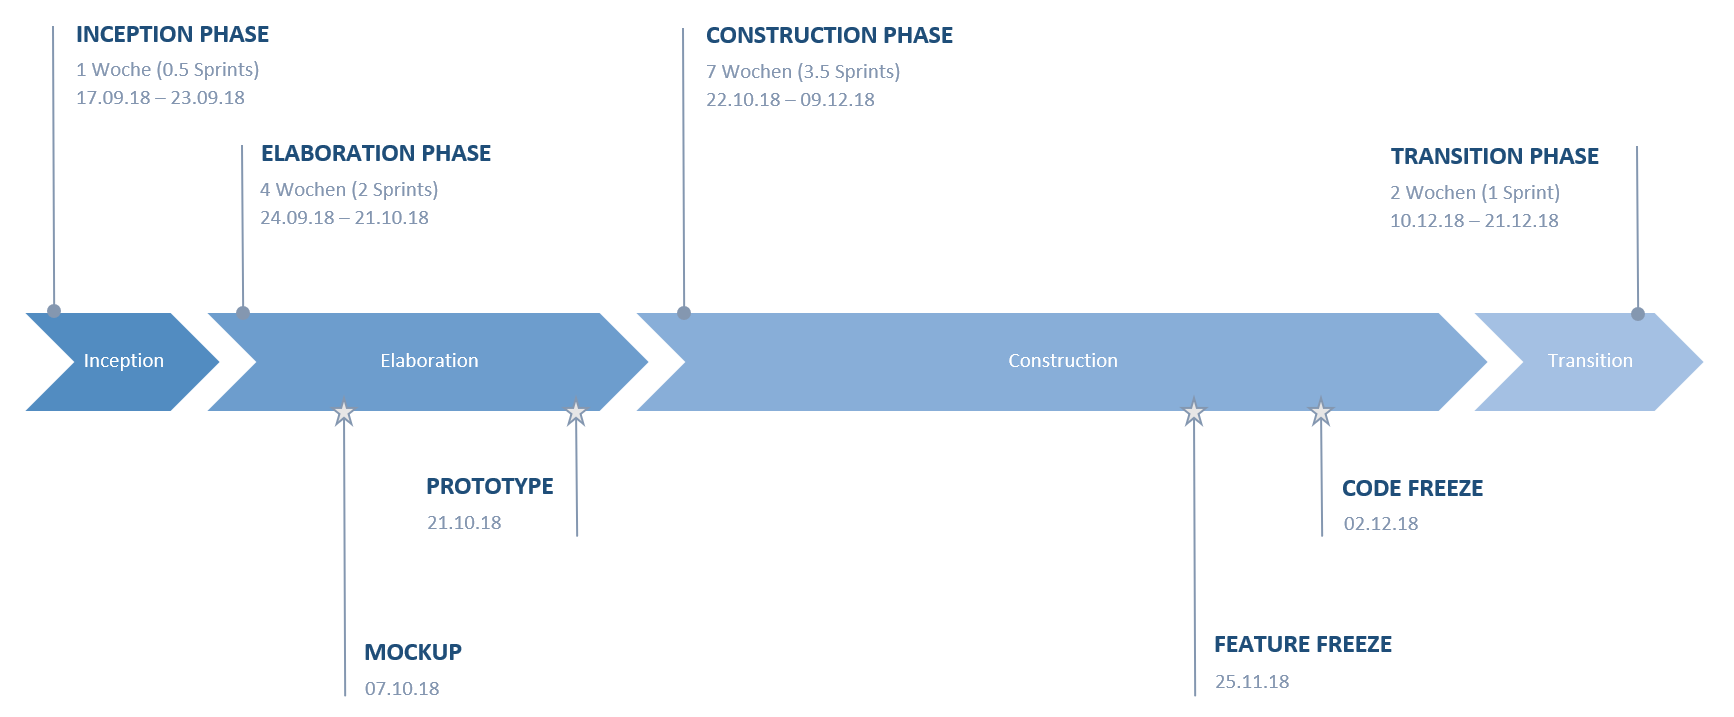
\includegraphics[width=1\linewidth, height=9.6cm]{img/projekt-plan/projekt-plan}
			\caption[Projektplan]{Projektplan}
			\label{fig:projekt-plan}
		\end{figure}
	\vspace{0.5cm}
	\subsection{Risikotabelle}\label{risiko-tabelle}
	
	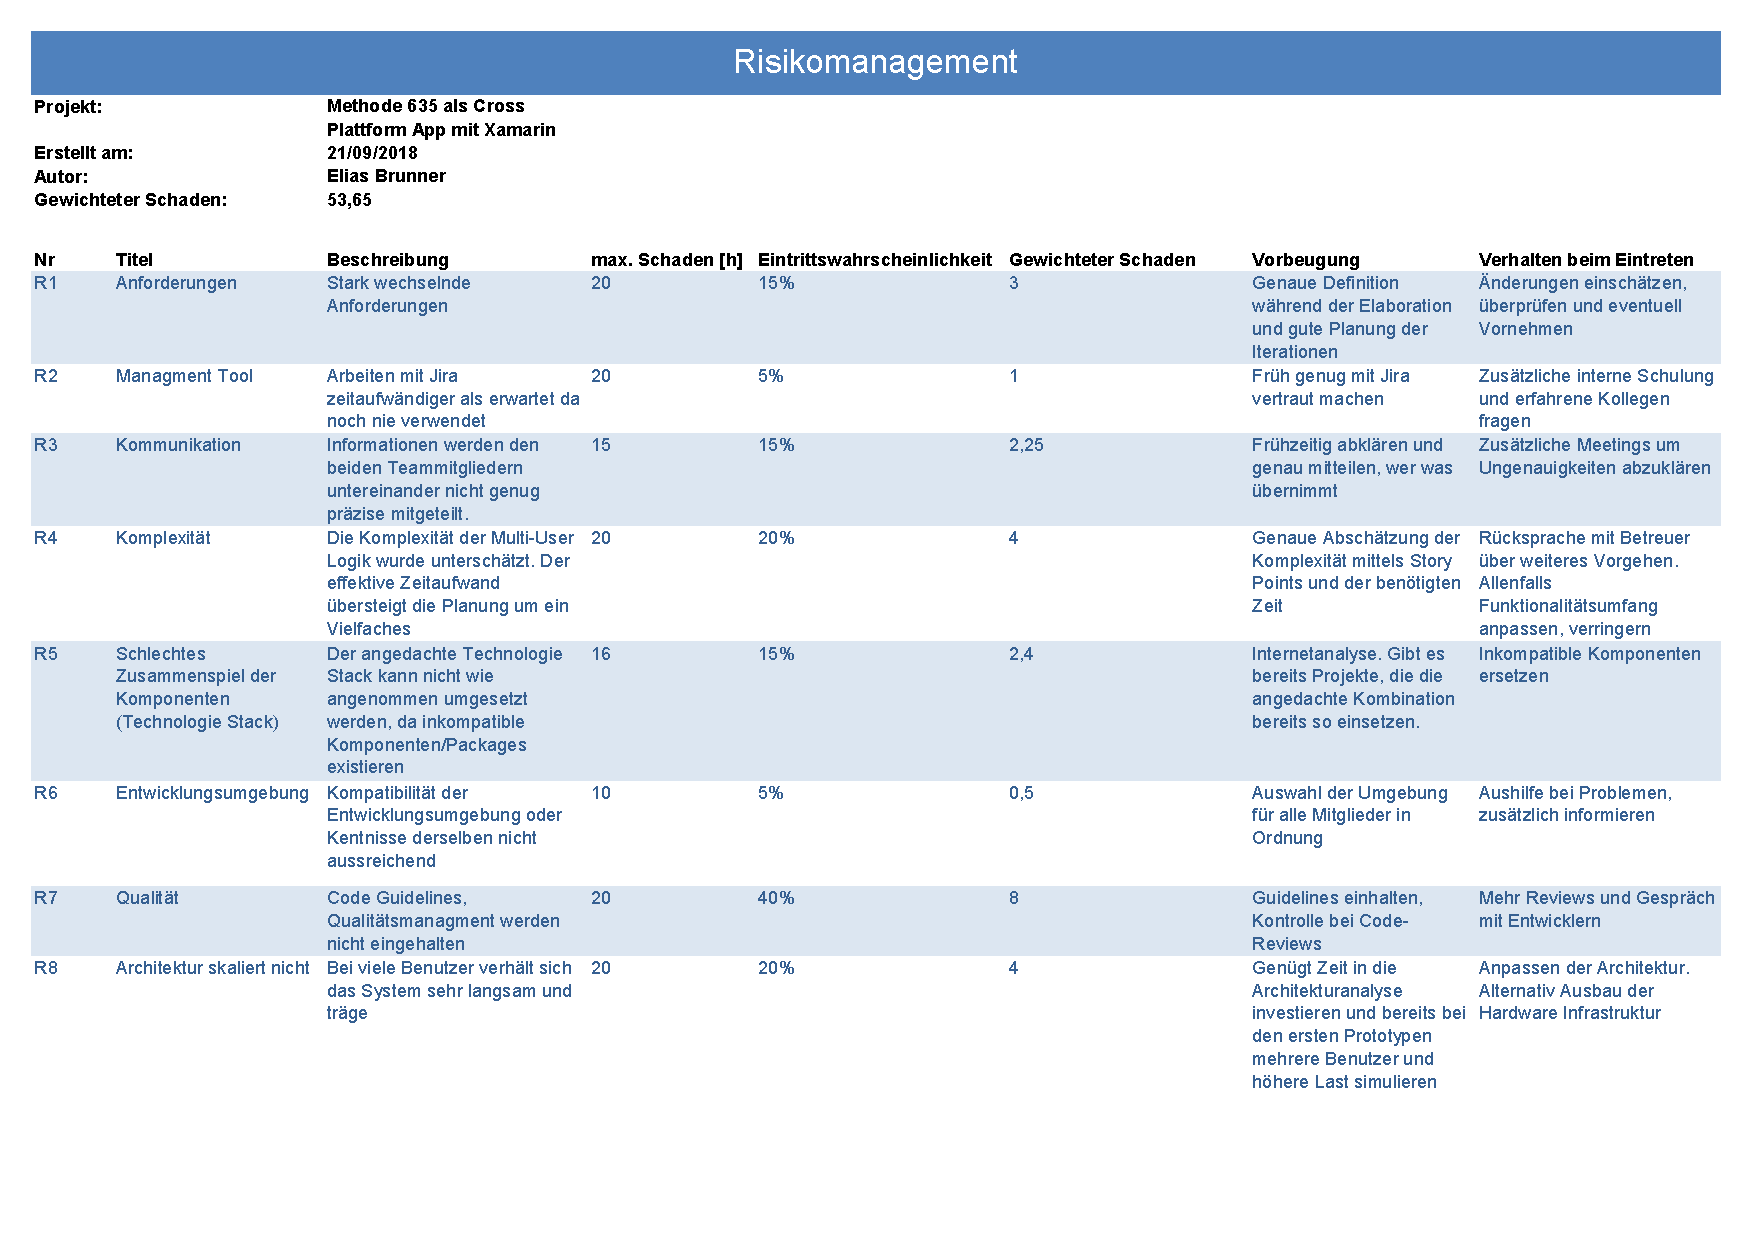
\includepdf[pages=-,landscape=true]{./res/projekt_risiko/TechnischeRisiken.pdf}
	\label{pdf:projekt-risiken}
	
\end{landscape}